\documentclass{article}

\usepackage{float}
\usepackage{multirow}
\usepackage{booktabs}
\usepackage{pgfplots}
\usepackage{hyperref}
\usepackage{cleveref}

\renewcommand{\axisdefaultheight}{190pt}
\newcommand*{\bigO}[1]{\ensuremath{\mathcal{O}\left(#1\right)}}

\title{Programming Assignment 1 Report}
\author{
    Hanlin He\footnote{\texttt{hxh160630@utdallas.edu}},
    Lizhong Zhang\footnote{\texttt{lxz160730@utdallas.edu}}
}
\date{\today}

\begin{document}
\maketitle

We run experiments using 24, 36 and 48 cores, with threads number ranging
from 2 up to the number of cores. Each experiment runs 20 to 30 times and the
average running times were used to minimize Java GC overhead.

\section*{Result \& Analysis}

Note: All time result is in millisecond.

\subsection*{24 Cores}
The experiment results for 24 cores are plotted in \cref{exp_plot_24} and detailed
results are shown in \cref{exp_table_24}.

\begin{figure}[H]
    \caption{Experiment Results 1}
    \label{exp_plot_24}
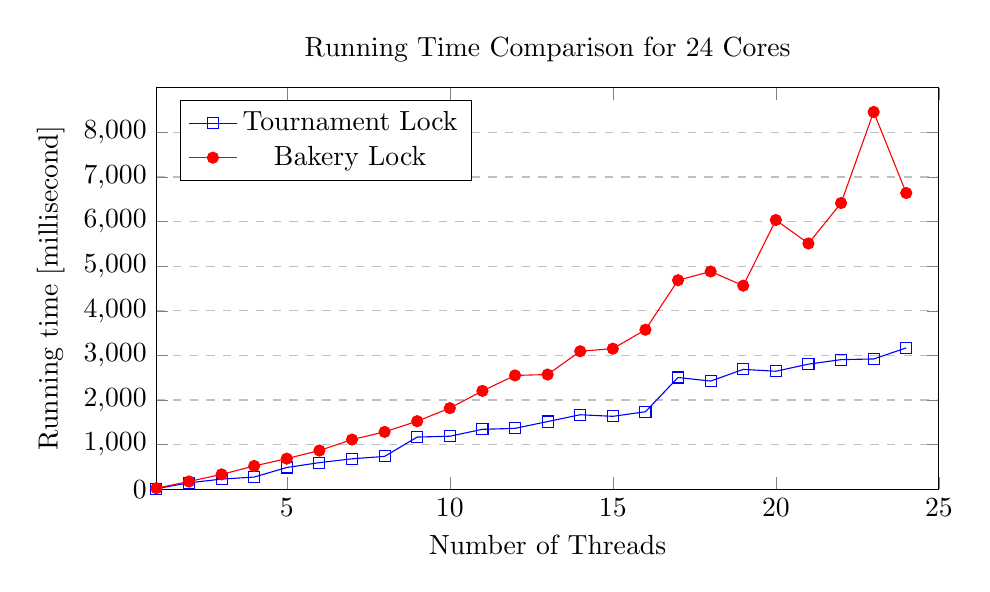
\begin{tikzpicture}
\begin{axis}[
    width=.95\textwidth,
    height=\axisdefaultheight,
    title={Running Time Comparison for 24 Cores},
    xlabel={Number of Threads},
    ylabel={Running time [millisecond]},
    xmin=1, xmax=25,
    ymin=0, ymax=9000,
    xtick={5,10,15,20,25},
    ytick={0,1000,2000,3000,4000,5000,6000,7000,8000},
    legend pos=north west,
    ymajorgrids=true,
    grid style=dashed,
]
\addplot[
    color=blue,
    mark=square,
    ]
    coordinates {
        (1,9.47)
        (2,141.67)
        (3,224.87)
        (4,271.00)
        (5,485.47)
        (6,594.07)
        (7,680.13)
        (8,733.93)
        (9,1168.13)
        (10,1186.33)
        (11,1341.60)
        (12,1363.13)
        (13,1516.07)
        (14,1668.33)
        (15,1632.87)
        (16,1735.53)
        (17,2504.00)
        (18,2423.40)
        (19,2686.07)
        (20,2644.20)
        (21,2803.60)
        (22,2904.60)
        (23,2919.47)
        (24,3168.27)
    };
\addplot[
    color=red,
    mark=*,
    ]
    coordinates {
        (1,21.27)
        (2,171.73)
        (3,331.07)
        (4,519.00)
        (5,683.73)
        (6,865.80)
        (7,1111.93)
        (8,1283.93)
        (9,1524.07)
        (10,1816.40)
        (11,2203.20)
        (12,2550.47)
        (13,2569.93)
        (14,3092.47)
        (15,3150.67)
        (16,3575.00)
        (17,4686.13)
        (18,4881.47)
        (19,4563.80)
        (20,6036.00)
        (21,5509.67)
        (22,6416.73)
        (23,8459.47)
        (24,6641.73)
    };
    \legend{Tournament Lock, Bakery Lock}
\end{axis}
\end{tikzpicture}
\end{figure}

\begin{table}[H]
    \caption{Result Detail of Lock Benchmark Experiment on 24 Cores}
    \label{exp_table_24}
    \centering
    \begin{tabular}{c|ll|c|ll}
        \toprule
        \multirow{2}{*}{Cores} & \multicolumn{2}{|c|}{Running Time} &
        \multirow{2}{*}{Cores} & \multicolumn{2}{|c}{Running Time} \\
                               & Tournament & Bakery & & Tournament & Bakery \\\midrule
        1 & 9.47 & 21.27 & 13 & 1516.07 & 2569.93 \\
        2 & 141.67 & 171.73 & 14 & 1668.33 & 3092.47 \\
        3 & 224.87 & 331.07 & 15 & 1632.87 & 3150.67 \\
        4 & 271.00 & 519.00 & 16 & 1735.53 & 3575.00 \\
        5 & 485.47 & 683.73 & 17 & 2504.00 & 4686.13 \\
        6 & 594.07 & 865.80 & 18 & 2423.40 & 4881.47 \\
        7 & 680.13 & 1111.93 & 19 & 2686.07 & 4563.80 \\
        8 & 733.93 & 1283.93 & 20 & 2644.20 & 6036.00 \\
        9 & 1168.13 & 1524.07 & 21 & 2803.60 & 5509.67 \\
        10 & 1186.33 & 1816.40 & 22 & 2904.60 & 6416.73 \\
        11 & 1341.60 & 2203.20 & 23 & 2919.47 & 8459.47 \\
        12 & 1363.13 & 2550.47 & 24 & 3168.27 & 6641.73 \\
        \bottomrule
    \end{tabular}
\end{table}


\subsection*{36 Cores}
The experiment results for 36 cores are plotted in \cref{exp_plot_36} and detailed
results are shown in \cref{exp_table_36}.

\begin{figure}[H]
    \caption{Experiment Results 2}
    \label{exp_plot_36}
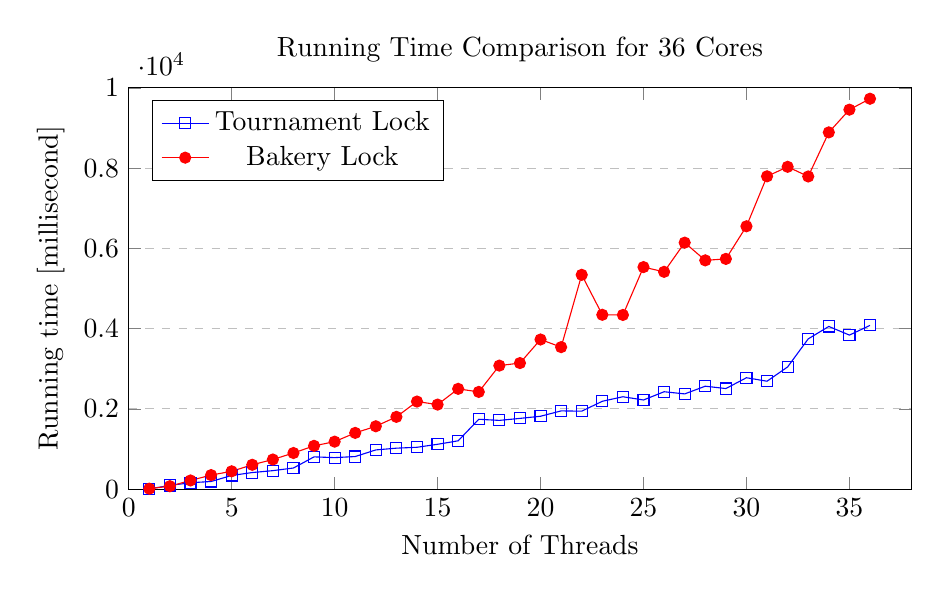
\begin{tikzpicture}
\begin{axis}[
    width=.95\textwidth,
    height=\axisdefaultheight,
    title={Running Time Comparison for 36 Cores},
    xlabel={Number of Threads},
    ylabel={Running time [millisecond]},
    xmin=0, xmax=38,
    ymin=0, ymax=10000,
    xtick={0,5,10,15,20,25,30,35},
    ytick={0,2000,4000,6000,8000,10000},
    legend pos=north west,
    ymajorgrids=true,
    grid style=dashed,
]
\addplot[
    color=blue,
    mark=square,
    ]
    coordinates {
        (1,6.60)
        (2,92.93)
        (3,159.33)
        (4,190.53)
        (5,341.33)
        (6,413.73)
        (7,461.07)
        (8,526.67)
        (9,804.47)
        (10,785.60)
        (11,812.33)
        (12,977.60)
        (13,1021.07)
        (14,1043.40)
        (15,1118.00)
        (16,1204.47)
        (17,1741.20)
        (18,1713.40)
        (19,1763.13)
        (20,1816.80)
        (21,1950.13)
        (22,1943.20)
        (23,2189.67)
        (24,2302.73)
        (25,2222.07)
        (26,2427.60)
        (27,2373.60)
        (28,2565.67)
        (29,2507.00)
        (30,2776.40)
        (31,2689.80)
        (32,3046.07)
        (33,3745.07)
        (34,4054.53)
        (35,3839.13)
        (36,4081.00)
    };
\addplot[
    color=red,
    mark=*,
    ]
    coordinates {
        (1,11.40)
        (2,73.93)
        (3,216.47)
        (4,350.33)
        (5,444.67)
        (6,606.87)
        (7,738.93)
        (8,900.73)
        (9,1079.13)
        (10,1183.53)
        (11,1401.87)
        (12,1566.93)
        (13,1801.40)
        (14,2183.13)
        (15,2106.93)
        (16,2499.47)
        (17,2423.20)
        (18,3078.87)
        (19,3142.20)
        (20,3729.67)
        (21,3539.20)
        (22,5340.87)
        (23,4345.07)
        (24,4341.00)
        (25,5533.87)
        (26,5415.40)
        (27,6143.00)
        (28,5701.27)
        (29,5737.87)
        (30,6550.80)
        (31,7795.73)
        (32,8032.87)
        (33,7792.00)
        (34,8891.00)
        (35,9457.13)
        (36,9729.13)
    };
    \legend{Tournament Lock, Bakery Lock}
\end{axis}
\end{tikzpicture}
\end{figure}

\begin{table}[H]
    \caption{Result Detail of Lock Benchmark Experiment on 36 Cores}
    \label{exp_table_36}
    \centering
    \begin{tabular}{c|ll|c|ll}
        \toprule
        \multirow{2}{*}{Cores} & \multicolumn{2}{|c|}{Running Time} &
        \multirow{2}{*}{Cores} & \multicolumn{2}{|c}{Running Time} \\
                               & Tournament & Bakery & & Tournament & Bakery \\\midrule
        1 & 6.60 & 11.40 & 19 & 1763.13 & 3142.20 \\
        2 & 92.93 & 73.93 & 20 & 1816.80 & 3729.67 \\
        3 & 159.33 & 216.47 & 21 & 1950.13 & 3539.20 \\
        4 & 190.53 & 350.33 & 22 & 1943.20 & 5340.87 \\
        5 & 341.33 & 444.67 & 23 & 2189.67 & 4345.07 \\
        6 & 413.73 & 606.87 & 24 & 2302.73 & 4341.00 \\
        7 & 461.07 & 738.93 & 25 & 2222.07 & 5533.87 \\
        8 & 526.67 & 900.73 & 26 & 2427.60 & 5415.40 \\
        9 & 804.47 & 1079.13 & 27 & 2373.60 & 6143.00 \\
        10 & 785.60 & 1183.53 & 28 & 2565.67 & 5701.27 \\
        11 & 812.33 & 1401.87 & 29 & 2507.00 & 5737.87 \\
        12 & 977.60 & 1566.93 & 30 & 2776.40 & 6550.80 \\
        13 & 1021.07 & 1801.40 & 31 & 2689.80 & 7795.73 \\
        14 & 1043.40 & 2183.13 & 32 & 3046.07 & 8032.87 \\
        15 & 1118.00 & 2106.93 & 33 & 3745.07 & 7792.00 \\
        16 & 1204.47 & 2499.47 & 34 & 4054.53 & 8891.00 \\
        17 & 1741.20 & 2423.20 & 35 & 3839.13 & 9457.13 \\
        18 & 1713.40 & 3078.87 & 36 & 4081.00 & 9729.13 \\
        \bottomrule
    \end{tabular}
\end{table}

\subsection*{48 Cores}
The experiment results for 48 cores are plotted in \cref{exp_plot_48} and
detailed results are shown in \cref{exp_table_48}.

\begin{figure}[H]
    \caption{Experiment Results 1}
    \label{exp_plot_48}
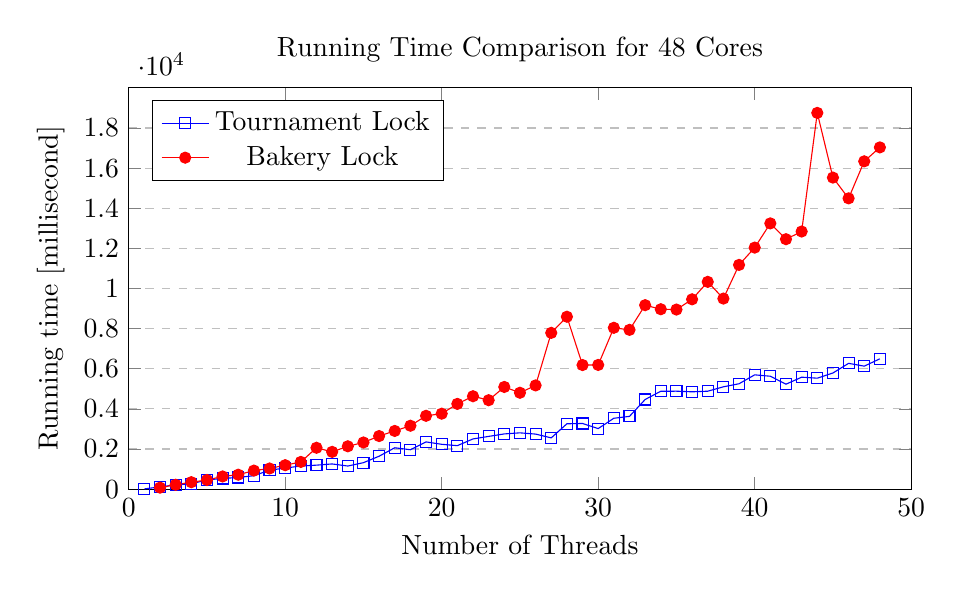
\begin{tikzpicture}
\begin{axis}[
    width=.95\textwidth,
    height=\axisdefaultheight,
    title={Running Time Comparison for 48 Cores},
    xlabel={Number of Threads},
    ylabel={Running time [millisecond]},
    xmin=0, xmax=50,
    ymin=0, ymax=20000,
    xtick={0,10,20,30,40,50},
    ytick={0,2000,4000,6000,8000,10000,12000,14000,16000,18000},
    legend pos=north west,
    ymajorgrids=true,
    grid style=dashed,
]

\addplot[
    color=blue,
    mark=square,
    ]
    coordinates {
        (1,12.30)
        (2,112.30)
        (3,212.40)
        (4,263.80)
        (5,461.90)
        (6,532.10)
        (7,581.40)
        (8,670.80)
        (9,945.90)
        (10,1051.70)
        (11,1152.60)
        (12,1196.60)
        (13,1256.00)
        (14,1152.10)
        (15,1319.80)
        (16,1641.10)
        (17,2062.70)
        (18,1965.50)
        (19,2354.20)
        (20,2235.00)
        (21,2167.20)
        (22,2503.40)
        (23,2628.80)
        (24,2753.00)
        (25,2806.20)
        (26,2744.10)
        (27,2555.50)
        (28,3258.80)
        (29,3272.30)
        (30,3018.20)
        (31,3532.90)
        (32,3628.10)
        (33,4468.50)
        (34,4880.10)
        (35,4882.30)
        (36,4851.60)
        (37,4881.70)
        (38,5100.50)
        (39,5252.70)
        (40,5697.80)
        (41,5627.20)
        (42,5231.10)
        (43,5580.90)
        (44,5531.10)
        (45,5789.60)
        (46,6270.10)
        (47,6130.00)
        (48,6496.10)
    };
\addplot[
    color=red,
    mark=*,
    ]
    coordinates {
        (2,75.27)
        (3,218.80)
        (4,346.73)
        (5,456.53)
        (6,632.60)
        (7,719.40)
        (8,924.60)
        (9,1030.13)
        (10,1193.87)
        (11,1356.93)
        (12,2061.93)
        (13,1857.33)
        (14,2135.60)
        (15,2326.87)
        (16,2646.33)
        (17,2901.00)
        (18,3160.40)
        (19,3654.80)
        (20,3761.20)
        (21,4249.40)
        (22,4631.13)
        (23,4433.40)
        (24,5093.67)
        (25,4804.00)
        (26,5170.53)
        (27,7789.40)
        (28,8593.53)
        (29,6185.13)
        (30,6191.47)
        (31,8042.40)
        (32,7939.00)
        (33,9169.60)
        (34,8967.07)
        (35,8950.40)
        (36,9461.40)
        (37,10331.40)
        (38,9498.00)
        (39,11176.47)
        (40,12038.40)
        (41,13246.00)
        (42,12458.40)
        (43,12840.73)
        (44,18753.47)
        (45,15528.53)
        (46,14493.67)
        (47,16339.20)
        (48,17033.67)
    };
    \legend{Tournament Lock, Bakery Lock}
\end{axis}
\end{tikzpicture}
\end{figure}

\begin{table}[H]
    \caption{Result Detail of Lock Benchmark Experiment on 48 Cores}
    \label{exp_table_48}
    \centering
    \begin{tabular}{c|ll|c|ll}
        \toprule
        \multirow{2}{*}{Cores} & \multicolumn{2}{|c|}{Running Time} &
        \multirow{2}{*}{Cores} & \multicolumn{2}{|c}{Running Time} \\
                               & Tournament & Bakery & & Tournament & Bakery \\\midrule
        2 & 100.80 & 75.27 & 26 & 2451.73 & 5170.53 \\
        3 & 181.20 & 218.80 & 27 & 2458.00 & 7789.40 \\
        4 & 192.67 & 346.73 & 28 & 2595.27 & 8593.53 \\
        5 & 333.80 & 456.53 & 29 & 2540.93 & 6185.13 \\
        6 & 384.00 & 632.60 & 30 & 2663.00 & 6191.47 \\
        7 & 464.00 & 719.40 & 31 & 2886.33 & 8042.40 \\
        8 & 510.07 & 924.60 & 32 & 3206.93 & 7939.00 \\
        9 & 801.40 & 1030.13 & 33 & 4052.20 & 9169.60 \\
        10 & 847.80 & 1193.87 & 34 & 3591.13 & 8967.07 \\
        11 & 876.53 & 1356.93 & 35 & 3697.07 & 8950.40 \\
        12 & 915.87 & 2061.93 & 36 & 3929.40 & 9461.40 \\
        13 & 1057.20 & 1857.33 & 37 & 3882.00 & 10331.40 \\
        14 & 1200.60 & 2135.60 & 38 & 4361.53 & 9498.00 \\
        15 & 1103.40 & 2326.87 & 39 & 4395.13 & 11176.47 \\
        16 & 1210.73 & 2646.33 & 40 & 4194.53 & 12038.40 \\
        17 & 1759.60 & 2901.00 & 41 & 4608.87 & 13246.00 \\
        18 & 1623.20 & 3160.40 & 42 & 4411.53 & 12458.40 \\
        19 & 1784.00 & 3654.80 & 43 & 4518.93 & 12840.73 \\
        20 & 1794.40 & 3761.20 & 44 & 4714.53 & 18753.47 \\
        21 & 1928.93 & 4249.40 & 45 & 4687.53 & 15528.53 \\
        22 & 1843.27 & 4631.13 & 46 & 4936.40 & 14493.67 \\
        23 & 2208.07 & 4433.40 & 47 & 5242.67 & 16339.20 \\
        24 & 2365.73 & 5093.67 & 48 & 4989.13 & 17033.67 \\
        \bottomrule
    \end{tabular}
\end{table}

\section*{Conclusion}

Based on our experiments, tournament lock's running time is approximately
\bigO{n}, where $n$ is the number of threads. Bakery lock's running time is longer than tournament lock, and closer
to \bigO{n^2}.

A side node: For our implementation, tournament lock works fine if the number
of threads is slightly larger than the number of cores, but the bakery lock's
performance would drop dramatically in such scenarios.

\end{document}
